\section{Introdução}

\textbf{RGPD} | Regulamento Geral de Proteção de dados, ou \textbf{GDPR}, é um tema bastante comum nos dias que correm, visto que foi necessário realizar a sua implementação nos mais diversos tipos de negócio. Este foi um dos projetos implementados na \textbf{UPI} e, este trabalho tem como objetivo analisar o impacto das diversas operações que o \textbf{RGPD} implica.

Assim sendo e, tendo como base o \textbf{Projeto A} realizado para esta unidade curricular,  é possível analisar ao longo deste relatório toda a informação sobre o projeto, bem como os diversos pontos analisados ao longo deste projeto.

\subsection{Objetivos do Projeto}

Este projeto tem como principal objetivo analisar o impacto das diversas operações de tratamento de dados, referidas no \textit{art.$^\circ$ 35} do \textbf{Regulamento Geral de Proteção de Dados} (\textif{\href{https://eur-lex.europa.eu/legal-content/PT/TXT/PDF/?uri=CELEX:32016R0679&from=EN}{Regulamento (UE) 2016/679}}).

Assim sendo, o principal resultado deste projeto prende-se com a elaboração de um \textbf{relatório técnico} com o diagnóstico da situação atual e um conjunto de possível recomendações, devidamente planeadas.

\subsection{Âmbito do Projeto}

O objetivo principal já referido anteriormente, porém existem outros pontos que são subentendidos ou adjacentes a este, sendo, como tal, importantes uma vez que visam explorar o âmbito do produto de forma mais completa. Sendo eles:

\begin{itemize}
	\item Identificação do impacto do \textbf{RGPD} sobre os processos organizacionais e Sistemas de Informação da \textbf{UPI};
	\item Identificação do nível de cumprimentos dos diferentes elementos afetados, com respeito aos requisitos e exigências estabelecidos pelo \textbf{RGPD};
	\item Identificação dos riscos a que se encontram expostos os tratamentos de dados relacionados com os diferentes processos organizacionais em que se decompõe a atividade da \textbf{UPI}, considerando os aspetos setoriais específicos da sua missão e atribuições;
	\item Definição de orientações, transversais a toda a \textbf{UPI}, para o cumprimento dos novos requisitos introduzidas pelo \textbf{RGPD}, tendo em consideração os diferentes fatores;
	\item Estabelecer os planos para o cumprimento dos requisitos do \textbf{RGPD} nas diferentes Unidades Orgânicas da \textbf{UPI}.
\end{itemize}

Lembrando que a \textbf{avaliação de impacto de privacidade} engloba todas as Unidades Orgânicas e Serviços da \textbf{UPI}.


\subsection{Fases do Projeto}

Este projeto divide-se em 4 fases principais, sendo elas:

\begin{center}
	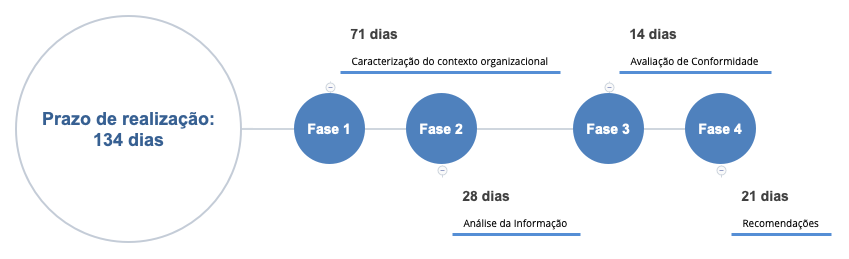
\includegraphics[width=1\textwidth]{fases}
	\captionof{figure}{Fases do projeto}
\end{center}

\begin{itemize}
	\item \textbf{Fase 1:} 
		\begin{itemize}
			\item Caracterização do contexto organizacional
			\item 71 dias
		\end{itemize}
	\item \textbf{Fase 2:}
		\begin{itemize}
			\item Análise da Informação
			\item 28 dias
		\end{itemize}
	\item \textbf{Fase 3:}
		\begin{itemize}
			\item Avaliação de conformidade
			\item 14 dias
		\end{itemize}
	\item \textbf{Fase 4:}
		\begin{itemize}
			\item Recomendações
			\item 21 dias
		\end{itemize}
\end{itemize}